
\chapter{Introduction}





\section{Muscle anatomy}

Movement is achieved using over 600 skeletal muscles, the ones that can be controlled voluntary. 

Smooth muscles - mostly in internal organs

cardiac muscle

Elementary building block of a muscle is muscle cell, or muscle fiber - \emph{myocyte}. Myocytes are ensheated by \emph{endomysium}, a connective tissue that contains nerves and capillaries. They are organized in bundles of 10 to 100, \emph{fascicles}, and surrounded by sheath of connective tissue, \emph{perymisium}. Group of fascicles is finally grouped together and enveloped by \emph{epimysium}, forming a muscle.

\emph{Sarcolema} is the cell membrane of myocyte, consisting of a lipid bilayer that contains intracelular liquid, \emph{myoplasma}. In the myoplasma, thin and thick filaments are serially connected, forming \emph{sarcomeres}, which are longitudinally connected in \emph{myofibrils} that extend through entire length of the myocyte. During shortening of muscle fibers, thin and thick filaments of sarcomeres are pulled together by cross-bridges between them. Total shortening of myofibril is summation of shortenings of sarcomeres of which it is composed.

Each motor neuron at the neuromuscular junction innervates several muscle fibers, forming the smallest functional unit called \emph{motor unit}. It was firstly defined by Liddell and Sherrington in 1925 \citep{Liddell1925, Sherrington1925} and is composed of motor neuron with axon and dendrites, and muscle fibers that axon innervates \citep{Duchateau2011}. Since motor neuron with a single action potential usually evokes action potentials simultaneously in all belonging muscle fibers, by observing action potentials of the muscle fibers, information on activity of motor neurons in spinal cord or brain stem can be inferred \citep{Merletti-Farina-book}. % mozda ne treba ovaj citat

Motor neurons transfer nerve impulses that control the muscle from spinal cord to neuromuscular junction. At the nerve endings action potentials trigger the release of the neurotransmitter \emph{acetylcholine} to the narrow space between the axon and sarcolema, which causes sodium channels in sarcolema to open. If the amount of acetylcoline is sufficient for the excitation, depolarization takes place and the action potential propagates longitudinally from the junction towards the ends of the fiber causing contraction \citep{Henneberg1999}. Speed of action potential propagation is called \emph{conduction velocity} and typically ranges around 4 m/s. 

Detailed analysis of muscle physiology can be found elsewhere \citep{Squire1986}.

Pool of motor neurons that innervates entire muscle generally ranges from ten to thousand, depending on the muscle. \citep{Merletti-Farina-book}.

By the characteristics of muscle fiber, there are three main types of muscle fibers:
\change{prepisi od Monice}
\begin{itemize}
\item Fast twitch, fatigable fibers (FF, or type IIb)\\
They have high levels of ATP for anaerobic energy supply. They are present in pale muscles. glycolytic and work well in ischemic or low oxygen conditions. fast twitch, large forces. high nerve conduction velocity. 
\item Fast twitch, fatigue-resistant (FR, or type IIa)
oxidative glycolytic, have fast twitch and are resistant to fatigue. intermediate conduction velocity 

\item Slow twitch, very resistant to fatigue (S, or type I)
Oxidative and do not work well in low oxygen conditions. They generate small forces, have slow twitch and resistant to fatigue. lower nerve conduction velocity. This fiber type is very resilient to fatigue because of high oxidative metabolism and energy efficiency. They are present in high percentage in red muscles, such as soleus.
\end{itemize}

Muscle fibers innervated by the same motor neuron have similar histochemical and contractile characteristics.

Force that muscle fibers generate depends on firing frequency of the action potentials (rate coding) innervating the neuromuscular junction, and the recruitment strategy by which the motor units are activated, i.e., the number of activated motor units. Firing frequency and the recruitment strategy depend on the speed and force of contraction. Muscle units with low threshold are activated firstly, resulting in low force and high endurance, i.e., resistance to fatigue. If greater force is required, muscle units with higher threshold that are prone to fatigue are activated \citep{Freund1975, Merletti-book}. This was first proposed by Henneman et al. in 1965 \citep{Henneman1965}, who state that order of recruitment of motor neurons is based on size principle, that is, neurons with smaller axons are recruited at lower effort levels and with increase in force, larger motoneurons are recruited. Therefore, S type muscle units, which have the smallest motoneurons are recruited first, followed by FR type units, and finally FF units. 



\section{Surface electromyography}

Myoelectric signal is a superposition of electrical activity (propagating action potentials) produced by the muscle fibers while contracting. It can be characterized
\citep{Farina2014}

EMG signals could be recorded either non-invasively (surface EMG, sEMG) or invasively with needle and wire electrodes (intramuscular EMG, iEMG) \citep{Marateb1999}. Although iEMG signal is usually with higher quality (in terms of signal-to-noise ratio), it was shown that both approaches provide a similar quality of identification of upper-arm motor task\citep{Hargrove2007}.

Depending on number of electrodes used for the recording. the following classification exists: monopolar, bipolar, linear electrode array, and high-density EMG (see Figure \ref{fig:electrode_types})

\begin{figure}[ht]
\centering
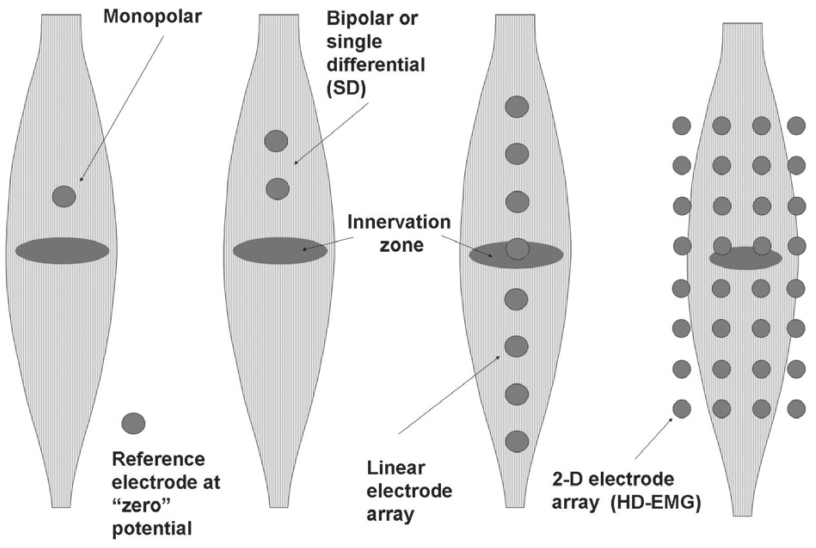
\includegraphics[width=0.5\textwidth]{Images/electrode_types.png}
\caption{Four types of recording surface EMG signal: monopolar, bipolar, linear electrode array, HD-EMG. Figure was modified from \citep{Merletti2010}
Traditional monopolar detection with respect to a remote reference taken as zero (reference) potential. b) Bipolar (or single differential, SD) detection (or mon- tage) along the fiber direction. c) Linear (one dimensional, 1-D) array of electrodes along the fiber direction. Spatial filters (such as double or N-differential) can be obtained by properly weighting and adding the signals from nearby electrodes. d) 2-dimensional (2-D) array of electrodes providing an image of potential distribution. Spatial filters (such as double or N-differential in the column or row direction, Laplacian, inverse binomial, etc.) may be applied to the signals. Image processing procedures may be applied to the “image” to interpolate or virtually rotate the image to align it with the fiber direction or to detect edges or areas of high or low activity or gradient.
are}
\label{fig:electrode_types}
\end{figure}


HD-EMG \ref{fig:HD-EMG}

\begin{figure}[ht]
\centering
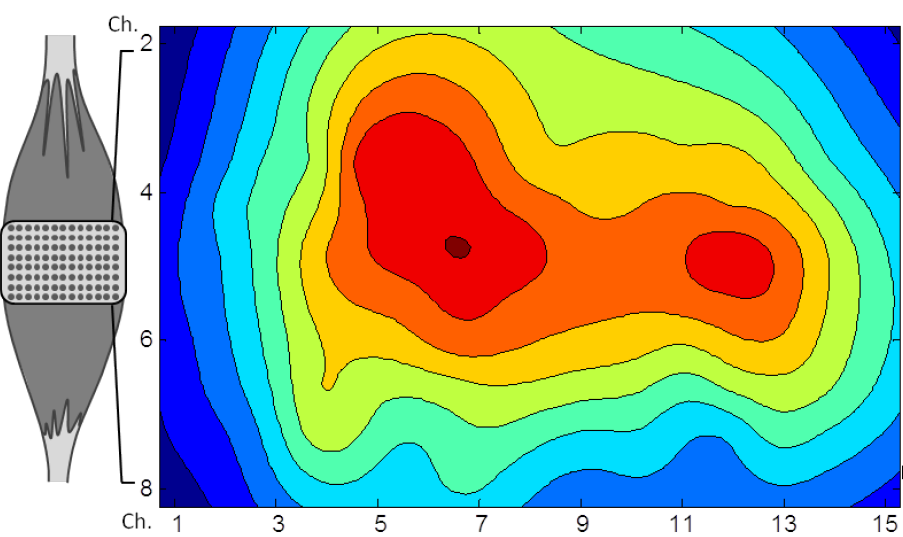
\includegraphics[width=0.95\textwidth]{Images/HD-EMG.png}
\caption{The figure represents the HD-EMG activation map recorded on the biceps brachii muscle during flexion. Distinct activation of the two heads can be noticed in the map. Modified from Monica}
\label{fig:HD-EMG}
\end{figure}


\section{Task identification}


The central nervous system (CNS) is responsible for processing information received from all parts of the body. The two main organs of the CNS are the brain and the spinal cord and are entirely composed of two kinds of specialized cells: neurons and glia. The brain is the most complex part of the human body and exerts a centralized control over the other organs. Neurons, the basic working units of the brain, are designed to transmit information within the brain to other nerve cells and to communicate with muscles and gland cells. The complex architecture of the brain is built on the extensive number of interconnected neurons sharing information through specialized connections called synapses. This connection allows  neurons to communicate through an electrical or chemical signals, producing ionic currents that generate electric and magnetic fields. 

The CNS is organized in multiple levels, from simple connections between cells to coordinated cell populations, building a complex architecture of interconnected brain regions. The neural processes at this last level are produced by the dynamic coordination of smaller elements. In the cerebral cortex, all this brain activity is summed and its electric and magnetic fields can be measured on the scalp surface. 



Pattern recognition is an alternative to conventional control algorithms. The prerequisite of using pattern recognition for task identification is the presence of a pattern that can be extracted from the EMG signal. Major advancement over conventional conventional switching myocontrol is the possibility of.

Pattern recognition approach doesn't support proportional and simultaneous control for multiple motor tasks. Therefore, tasks need to be performed sequentially. This type of control prevents the user from achieving a fluid movement, but also demands planning of movement execution. Although pattern recognition improves the possibility, it has serious limitations. 

This implies sequential control which prevents the subject from doing fluent, e.g. Davidge et al. designed a system where movements that combine DoFs are labeled as unique classes in LDA problem, whereas Young et al. \citep{Young2013} propose system of parallel LDA classifiers that use conditional probabilities to separate between combination of tasks.

Proportional review \citep{Fougner2012}
Force can be estimated based on the EMG : \citep{Staudenmann2010}

In pattern recognition, there is still a large gap between industry and practice \citep{Jiang2012}.

On the other hand, one of the disadvantages of pattern recognition is the fact that in spite of the high accuracy, an error could lead to the completely unwanted task. Also, although identification rate is usually very high during the stationary task, errors often occur during transition between tasks. This problems can be partially prevented by employing the e.g. majority voting principle \citep{Englehart2003} (300ms, LDA), or decision-based velocity ramp that attenuates the velocity of a movement after the change of a task \citep{Simon2011}. 

Challenges in pattern recognition are electrode shift \citep{Hargrove2008, Young2011}, change in arm posture \citep{Fougner2011}, slow time dependent changes \citep{Farina2014} such as fatigue \citep{Tkach2010}, and change in electrode-skin impedance \citep{Clancy2002a}.


Future works: dynamic system, hybrid system

\subsection{Pattern recognition}

Pattern recognition is a classification technique and the principle by which it is performed is learned independently from the data, i.e., training set. There are two main types of pattern recognition: supervised and unsupervised. Supervised pattern recognition implies that the classes of the training set are known and are used to obtain the model. New inputs are identified as one of the predetermined classes. On the other hand, unsupervised pattern recognition is used when no labels are available and samples are assigned to unknown classes. This technique is more appropriate for the clustering problem because the classes are determined automatically by the system, whereas supervised approach is more appropriate for the classification because classes are defined by the system designer, and, therefore, it is usually used in task identification based on EMG.

In statistical pattern recognition, each sample is composed of $m$ measures that form the pattern, i.e., features $(x_0, x_1, \dots, x_{m-1})$. The objective of the algorithm is to obtain a decision rule, i.e., the decision boundary which separates well samples of different classes. There are many \emph{state-of-the-art} classifiers that use various principles to construct these boundaries. However, many researchers agree that the fidelity of the classification in EMG applications depends mostly on selection of features. In other words, with appropriate selection of features, all classifiers will give similar classification result. A short introduction is provided on the two methods used in the thesis: Linear Discriminant Analysis and Support Vector Machine.


\subsubsection{Linear Discriminant Analysis}

\begin{myquote}
\begin{flushright}
\textit{All models are wrong; some models are useful.} \\George E. P. Box
\end{flushright}
\end{myquote}

Linear Discriminant Analysis is a computationally simple and efficient classifier with linear decision boundary and it is based on the Bayesian equation. In a classical problem with $n$ samples in training set, which consist of $m$ features, the dataset of available samples is a matrix of dimension $[n \times m]$, whereas the label that describes the belonging of each sample to one of the classes is $y$, where $y \in (0,1,2,...,K-1)$.

According to Bayesian equation, the probability that a sample $\mathbf{x}_0$ belongs to a class $k$ is equivalent to the: 
\begin{equation} 
P(y=k \,\, | \, \mathbf{x}=\mathbf{x}_0) = \frac{P(\mathbf{x}=\mathbf{x}_0  \,\, | \, y=k) \,\,P(y=k)} {P(\mathbf{x}=\mathbf{x}_0)}
\end{equation}

\noindent
, where k represents the class. Term $P(\mathbf{x}=\mathbf{x}_0  \,\, | \, y=k)$ is called the \emph{class-conditional} probability and describes the probability that the sample with exact features $\mathbf{x}_0$ is encountered within the group of samples belonging to the class $k$. Term $P(y=k)$ is called the \emph{a priori} probability and describes the probability that the sample belonging to the class $k$ is found within the group of all samples, regardless of the features. Finally, the term $P(\mathbf{x}=\mathbf{x}_0)$ is called the \emph{marginal} probability and describes the probability of finding the sample with exact set of features in the dataset, regardless of the class. Marginal probability can be written as a sum of class-conditional probabilities multiplied by the a priori probabilities for each class:

\begin{equation}
\begin{split}
P(\mathbf{x}=\mathbf{x}_0) = P(\mathbf{x}=\mathbf{x}_0  \,\, | \, y=1) \,\,P(y=1) + \\
P(\mathbf{x}=\mathbf{x}_0  \,\, | \, y=2) \,\,P(y=2) + \dots + \\
P(\mathbf{x}=\mathbf{x}_0  \,\, | \, y=K) \,\,P(y=K)
\end{split}
\end{equation}


Following the Bayesian theory, the hypothesis, i.e., the predicted class of a sample $\mathbf{x}_0$ is chosen as the class which has the highest probability $P(y=k \,\, | \, \mathbf{x}=\mathbf{x}_0)$:

\begin{equation} 
h(\mathbf{x}_0) = \argmax_k P(y=k \,\, | \, \mathbf{x}=\mathbf{x}_0)
\end{equation}

Statistically speaking, this is the best possible classifier. The problem arises in the implementation. The exact probability density functions are unknown and have to be estimated from the available data, which is the source of error.
Estimated version of the stated probabilities will be marked with a different symbols to stress out the fact they are just an estimates:

\begin{equation} 
p_k(\mathbf{x}) \coloneqq P(y=k \,\, | \, \mathbf{x})
\end{equation}

\begin{equation} 
g_k(\mathbf{x}) \coloneqq P(\mathbf{x}  \,\, | \, y=k)
\end{equation}

\begin{equation} 
\pi_k \coloneqq P(y=k)
\end{equation}


Linear Discriminant Analysis estimates marginal probability term ($\pi_k$) as a ratio of number of samples belonging to class $k$ and the total  number of samples, whereas the class-conditional probability term in the Bayesian equation is estimated as a multivariate Gaussian function:

\begin{equation} 
g_k(\mathbf{x}) = \frac{1}{(2 \pi)^{\nicefrac{m}{2}}\, |\Sigma_k|^{\nicefrac{1}{2}}}\,\, e^{\nicefrac{-1}{2}  (\mathbf{x}-\mu_k)^T  \Sigma_k^{-1} (\mathbf{x}-\mu_k)} 
\end{equation}

\noindent
, where $m$ is the dimensionality of the feature space, i.e., number of features representing each sample. Function $g_k$ is estimated class-conditional probability of class $k$, and $\mu_k$ and $\Sigma_k$ are the mean and co-variance matrix for class $k$, respectively, and they are estimated from the available data as:

\begin{equation}
\left. \mu_k = \frac{1}{n_k} \sum_{i}{\mathbf{x}_i} \right\vert_{\forall \mathbf{x} \in k}
\end{equation}

\begin{equation}
\left. \Sigma_k = \frac{1}{n_k-K} \sum_{i}{\Big( \mathbf{x}_i - \mu_k \Big) \Big( \mathbf{x}_i - \mu_k \Big)^T} \right\vert_{\forall \mathbf{x} \in k}
\end{equation}

 
\noindent
, where $n_k$ represents the number of samples belonging to a class $k$.
To simplify the model, LDA assumes that the co-variance matrices $\Sigma_k$ are the same for all classes:

\begin{equation} 
\Sigma_0 = \Sigma_1 = \dots = \Sigma_{K-1} = \Sigma
\end{equation}

\noindent
and they are usually calculated using the weighted average:
\begin{equation} 
\Sigma = \frac{\sum_{k=1}^K {n_k\Sigma_k}}{\sum_{k=1}^K{n_k}}
\end{equation}

\noindent
The consequence of this assumption is the linearity of the decision boundary. Without this assumption the same calculus would lead to quadratic discriminant analysis, which has non-linear boundary.

In a two class example ($y \in \{0,1\}$), all samples on the decision boundary will have the same probability of belonging to class 0 or 1:

\begin{equation} 
D.B. = \Big\{\mathbf{x}\,\, \Big| \,\,P\big(y=0 \, \big| \, \mathbf{x}=\mathbf{x}_0\big) = P\big(y=1 \, \big| \, \mathbf{x}=\mathbf{x}_0\big) \Big\}
\end{equation}

Following this idea, the decision boundary can be estimated by solving the equation:

\begin{equation} 
\frac{g_0(\mathbf{x}) \, \pi_0} {\cancel{\sum_{k=1}^K{g_k \, \pi_k}}} = \frac{g_1(\mathbf{x}) \, \pi_1} {\cancel{\sum_{k=1}^K{g_k \, \pi_k}}}
\end{equation}


\begin{equation} 
%\begin{split}
\frac{1}{(2 \pi)^{\nicefrac{m}{2}}\, |\Sigma_0|^{\nicefrac{1}{2}}}\,\, e^{\nicefrac{-1}{2}  (\mathbf{x}-\mu_0)^T  \Sigma_0^{-1} (\mathbf{x}-\mu_0)}  \,\,\,\pi_0 = \\
\frac{1}{(2 \pi)^{\nicefrac{m}{2}}\, |\Sigma_1|^{\nicefrac{1}{2}}}\,\, e^{\nicefrac{-1}{2}  (\mathbf{x}-\mu_1)^T  \Sigma_1^{-1} (\mathbf{x}-\mu_1)}  \,\,\,\pi_1
%\end{split}
\end{equation}

%,where $d$ is the dimensionality of the feature space, i.e., number of features representing each sample.
If making the assumption on the equal co-variance matrices for both classes $(\Sigma_0 = \Sigma_1  = \Sigma)$, and taking the logarithm, the equation takes the form: 
%\begin{equation} 
%\Sigma_0 = \Sigma_1  = \Sigma
%\end{equation}


\begin{equation} 
%\begin{split}
-\frac{1}{2}  \Big(\mathbf{x}-\mu_0\Big)^T  \Sigma^{-1} \Big(\mathbf{x}-\mu_0\Big) +  \log{\Big(\pi_0\Big)}= \\
-\frac{1}{2}  \Big(\mathbf{x}-\mu_1\Big)^T  \Sigma^{-1} \Big(\mathbf{x}-\mu_1\Big) +  \log{\Big(\pi_1\Big)}
%\end{split}
\end{equation}

, which can be written in the form of the linear function $x^T\beta + \alpha = 0$ as:

\begin{equation} 
\begin{split}
\mathbf{x}^T\Big(\Sigma^{-1} \mu_0 - \Sigma^{-1} \mu_1\Big) + \frac{1}{2} \Big(\mu_1^T \Sigma^{-1}\mu_1 - \mu_0^T \Sigma^{-1}\mu_0\Big)
+ \log\Big( \frac{\pi_0}{\pi_1}  \Big) = 0
\end{split}
\end{equation}

This equation represents the decision boundary between two classes, i.e., all samples lying on this line will have equal probability of belonging to class 0 and class 1. It should be noted that the slope of the line depends only on the class means and co-variance matrix, whereas a priori probabilities (which are the result of number of samples belonging to class 0 or 1) have effect only on the $y$-intercept term, i.e., the offset of the function. This is an interesting point that demands caution. If groups are unbalanced, that is, number of samples of one group is higher than in the other group, $y$-intercept of the decision boundary will be affected and the classifier will be biased by this disproportion. If groups are unbalanced because of the incomplete or missing data, whereas in reality they are balanced, this can have a negative effect.

When considering multiclass classification problem, probability of a sample belonging to each class is firstly estimated by the equation:

\begin{equation}
p_k = -\frac{1}{2} \log \big\vert \Sigma \big\vert - \frac{1}{2}  \Big(\mathbf{x}-\mu_k\Big)^T  \Sigma^{-1} \Big(\mathbf{x}-\mu_k\Big) +  \log{\Big(\pi_k\Big)}
\end{equation}

\noindent and then the class is estimated as the one with the highest probability as:

\begin{equation} 
h(\mathbf{x}) = \argmax_k p_k(\mathbf{x})
\end{equation}


\subsubsection{Support Vector Machine}

\begin{myquote}
\begin{flushright}
\textit{Try to solve the problem directly and never solve a more general problem as an intermediate step.} \\Vladimir Vapnik
\end{flushright}
\end{myquote}


Support vector machine is nowadays known as a very powerful classifier with a lot of different applications. The big advantage over LDA is the fact that it is a \emph{non-parametric} classifier. The model is not obtained using assumptions of the form of the class density function and estimation of it's parameters, which is inevitably erroneous. Instead, SVM forms the decision boundary using the samples (not their density estimates) by maximizing the distance between samples and the boundary.
This was the idea Vladimir Vapnik, the inventor of this method stood for. It is better to try to solve the problem directly and simply, without many intermediate steps that can be complicated and inaccurate.

%This classification method essentially has a very simple principle, but using several mathematical tricks, it became a very powerful tool. 

In pattern recognition, the decision rule ($h$) is usually obtained by multiplying the sample ($\mathbf{x}$) by predefined weights ($\Theta$):

\begin{equation} 
\Theta^T \mathbf{x} + \Theta_0
\end{equation}

\noindent , where $\Theta_0$ is a constant. If samples $\mathbf{x}_0$ and $\mathbf{x}_1$ lay on the decision boundary, following statements are true:

\begin{equation} 
\Theta^T \mathbf{x}_0 + \Theta_0 = \Theta^T \mathbf{x}_1 + \Theta_0
\end{equation}

\begin{equation} 
\Theta^T (\mathbf{x}_0 - \mathbf{x}_1) = 0
\end{equation}

\noindent This result implies that $\Theta$ is perpendicular to the boundary:
\begin{equation} 
\Theta \perp \left(\mathbf{x}_0 - \mathbf{x}_1\right)
\end{equation}


The goal of the SVM is to find the decision boundary between two classes so that the distance between the samples and the decision boundary, i.e., the margin is maximized. The distance ($d$) from a sample to the decision boundary can be defined as the distance between the sample $\mathbf{x}$ and any point lying on the boundary, $\mathbf{x}_0$, projected onto the vector $\Theta$.

\begin{equation} 
d = \frac{\Theta^T \big(\mathbf{x} - \mathbf{x}_0\big)}{\big\vert \Theta \big\vert}
\end{equation}

\noindent Term $\vert \Theta \vert$ is introduced to normalize the vector $\Theta$. Without the normalization the distance would depend on the norm of $\Theta$.

Since $\mathbf{x}_0$ is on the decision boundary, the expression $\Theta^T \mathbf{x}_0 + \Theta_0 = 0$ is valid, and, therefore, the expression for the distance can be written as:
\begin{equation} 
d = \frac{\Theta^T \mathbf{x} + \Theta_0}{\big\vert \Theta \big\vert}
\end{equation}

Margin ($M$) can be defined as the distance from the boundary to the closest sample:
\begin{equation} 
M = \min_i d_i
\end{equation}

Depending on which side of the boundary the sample is located, the distance can be positive or negative. In order to keep it strictly positive, term $y$ is introduced, where $y \in \{-1,1\}$:
\begin{equation} 
M = \min_i \big\{y_id_i\big\}
\end{equation}

\begin{equation} 
M = \min_i \left\{ \frac{y_i \left(\Theta^T \mathbf{x}_i + \Theta_0\right)}{\left\vert \Theta \right\vert} \right\}
\end{equation}

The objective is to maximize the margin $M$. Since $\Theta$ can be rescaled, a certain $\Theta$ exists so that $y_i \left(\Theta^T \mathbf{x}_i + \Theta_0\right) = 1$, which implies
\begin{equation} 
\exists \Theta, \,\, y_i \left(\Theta^T \mathbf{x}_i + \Theta_0\right) = 1 \,\,\,\, \Rightarrow \,\,\,\, M = \min_i \left\{ \frac{1}{\left\vert \Theta \right\vert} \right\}
\end{equation}

\noindent Therefore, to maximize the margin, a separating hyperplane should be found such that a norm of vector orthogonal to the hyperplane ($\Theta$) is minimal. 

For every point not on the boundary the following term is valid:
\begin{equation} 
y_i \left(\Theta^T \mathbf{x}_i + \Theta_0\right) > 0 
\end{equation}

Value $C$ can be selected such that:
\begin{equation} 
y_i \left(\Theta^T \mathbf{x}_i + \Theta_0\right) > C
\end{equation}

\begin{equation} 
y_i \left(\frac{\Theta^T \mathbf{x}_i}{C} + \frac{\Theta_0}{C}\right) > 1
\end{equation}

Since $\Theta$ and $\Theta_0$ can be rescaled, it can be written:
\begin{equation} 
\Theta := \frac{\Theta}{C}, \,\,\,\,\,\, \Theta_0 := \frac{\Theta_0}{C}
\end{equation}
%\begin{equation} 
%\Theta_0 := \frac{\Theta_0}{C}
%\end{equation}

\begin{equation} 
 y_i \left(\Theta^T \mathbf{x}_i + \Theta_0\right) > 1
\end{equation}

Finally the optimization problem states:

\begin{equation} 
\min \frac{1}{2} \vert \Theta \vert ^2, \,\,\,\, s.t. \,\,\, y_i \left(\Theta^T \mathbf{x}_i + \Theta_0\right) > 1.
\end{equation}

\noindent $L_2$ norm is preferred because it has continuous derivative, whereas constant $\nicefrac{1}{2}$ is introduced for the mathematical convenience. The optimization is solved using Lagrangian method as:

\begin{equation} \label{eq:SVM-opt}
L(\Theta, \Theta_0, \alpha_i) = \frac{1}{2} \vert \Theta \vert ^2 - \sum_{i=1}^n \alpha_i \left[y_i \left(\Theta^T \mathbf{x}_i + \Theta_0\right) - 1\right]
\end{equation}

\begin{equation} \label{eq:SVM-primal}
\frac{\partial L}{\partial \Theta} = \Theta - \sum_{i=1}^n \alpha_i y_i \mathbf{x}_i = 0 \,\,\,\, \Rightarrow \,\,\,\, \Theta = \sum_{i=1}^n \alpha_i y_i \mathbf{x}_i
\end{equation}

\begin{equation} \label{eq:SVM-dual}
\frac{\partial L}{\partial \Theta} = \sum_{i=1}^n \alpha_i y_i = 0
\end{equation}

By rewriting the problem in \ref{eq:SVM-opt} in terms of dual variable $\alpha$, the following expression can be obtained:

\begin{equation} 
L(\alpha) = \sum_i \alpha_i - \frac{1}{2} \sum_j \sum_i \alpha_j \alpha_i y_j y_i \mathbf{x}_i^T \mathbf{x}_j
\end{equation}

Since this function depends only on dual variable $\alpha$, the solution can be obtained by maximization:
\begin{equation} 
%\max \sum_i \alpha_i - \frac{1}{2} \sum_j \sum_i \alpha_j \alpha_i y_j y_i \mathbf{x}_i^T \mathbf{x}_j, \,\,\,\, s.t. \,\,\, \alpha_i \geq 0, \sum_i \alpha_i y_i = 0
%\max L(\alpha) \,\,\,\,\, s.t. \,\,\, \alpha_i \geq 0,   \sum_i \alpha_i y_i = 0
\max L(\alpha) \,\,\,\,\, s.t. \,\,\, \left\{\begin{array}{lr} \alpha_i \geq 0 \\
\sum_{i} \alpha_i y_i = 0  \end{array}\right.
\end{equation}

In this optimization problem, the objective has the form of quadratic function, whereas constraints are linear. This problem is typically solved using quadratic programming. Since it is a convex problem, the solution will always be global maximum. Once the dual variable $\alpha$ is found, the primal variable $\Theta$ can be calculated using the equation \ref{eq:SVM-primal}.

In the optimization, Karush-Kuhn-Tucker conditions need to be satisfied \citep{Boyd2004}. One of this condition is \emph{complementary slackness}, stating that in the optimal point (the solution of the problem), the product of dual variable and the constraint must be zero:
\begin{equation} 
\alpha_i \left[ y_i \left( \Theta^T\mathbf{x}_i + \Theta_0  \right) -1 \right] = 0
\end{equation}

This condition explains well the principle of SVM. Since the dual variable must be greater or equal to zero ($\alpha \geq 0$), there are two possibilities:
\begin{enumerate}
\item
If $\alpha$ is greater than zero, $\left[ y_i \left( \Theta^T\mathbf{x}_i + \Theta_0  \right) -1 \right]$ must equal one:
\begin{equation} 
\alpha_i > 0 \,\,\,\,\, \Rightarrow \,\,\,  y_i \left( \Theta^T\mathbf{x}_i + \Theta_0  \right) = 1
\end{equation}
\item
If $\left[ y_i \left( \Theta^T\mathbf{x}_i + \Theta_0  \right) -1 \right]$ is greater than zero, $\alpha$ must be zero:
\begin{equation} 
y_i \left( \Theta^T\mathbf{x}_i + \Theta_0  \right) > 1 \,\,\,\,\, \Rightarrow \,\,\,  \alpha = 0
\end{equation}
\end{enumerate}

Since for all samples lying on the margin, the statement  
\begin{equation}
y_i \left( \Theta^T\mathbf{x}_i + \Theta_0  \right) = 1
\end{equation}
\noindent holds, $\alpha$ will be greater than zero only for the samples lying on the decision hyperplane, whereas for the samples further away from the hyperplane, $\alpha$ will be zero. Given the fact that $\Theta$ depends on linear combination of samples weighted by $\alpha$ (eq. \ref{eq:SVM-primal}), only the samples lying on the boundary will have effect in the calculation of $\Theta$ (where $\alpha > 0$), and they are called \emph{support vectors}. This can be especially useful for the outlier samples.

The optimization problem does not depend on $\mathbf{x}$, but on $\mathbf{x}^T\mathbf{x}$. This allows the use of \emph{kernel trick} and implicitly enables nonlinear transform of the feature space at little additional cost. Usually, non-linear decision boundary can be achieved by nonlinear transform of features:
\begin{equation} 
\mathbf{x} \rightarrow \Phi(\mathbf{x})
\end{equation}

However, this operation is computationally expensive. The solution can be achieved using kernel functions. Kernel is a function $K(x,y)$ for which:
\begin{equation} 
K(\mathbf{x},\mathbf{y}) = \Phi(\mathbf{x})^T  \Phi(\mathbf{y})
\end{equation}

Since in the equation \ref{eq:SVM-dual} $\mathbf{x}$ does not appear by itself, but in a form of dot product $\mathbf{x}^T\mathbf{x}$, non-linear transform can be used in a form of kernel trick:
\begin{equation} 
L(\alpha) = \sum_i \alpha_i - \frac{1}{2} \sum_j \sum_i \alpha_j \alpha_i y_j y_i K(\mathbf{x}_i, \mathbf{x}_j)
\end{equation}

Most often used kernel is a radial basis kernel ($K_{RBF}(\mathbf{x}_i,\mathbf{x}_j)$):
\begin{equation} 
K_{RBF}(\mathbf{x}_i,\mathbf{x}_j) = e^\frac{-\parallel \mathbf{x}_i - \mathbf{x}_j\parallel^2}{2\sigma^2}
\end{equation}

Although SVM is conceptually designed as a two-class classifier, techniques for multiclass classification also exist, e.g. \emph{one-versus-one} or \emph{one-versus-all}.



\

